\documentclass{article} % For LaTeX2e
\usepackage{iclr2019,times}
\usepackage{amssymb}
\usepackage{float}
\usepackage{hyperref}
\usepackage{url}
\usepackage{bm}
\usepackage{graphicx,array} \graphicspath{{figures/}}
\usepackage{amsmath}
\usepackage{color}
\usepackage{caption}
\usepackage{subcaption}

% % Optional math commands from https://github.com/goodfeli/dlbook_notation.
% %%%%% NEW MATH DEFINITIONS %%%%%

\usepackage{amsmath,amsfonts,bm}

% Mark sections of captions for referring to divisions of figures
\newcommand{\figleft}{{\em (Left)}}
\newcommand{\figcenter}{{\em (Center)}}
\newcommand{\figright}{{\em (Right)}}
\newcommand{\figtop}{{\em (Top)}}
\newcommand{\figbottom}{{\em (Bottom)}}
\newcommand{\captiona}{{\em (a)}}
\newcommand{\captionb}{{\em (b)}}
\newcommand{\captionc}{{\em (c)}}
\newcommand{\captiond}{{\em (d)}}

% Highlight a newly defined term
\newcommand{\newterm}[1]{{\bf #1}}


% Figure reference, lower-case.
\def\figref#1{figure~\ref{#1}}
% Figure reference, capital. For start of sentence
\def\Figref#1{Figure~\ref{#1}}
\def\twofigref#1#2{figures \ref{#1} and \ref{#2}}
\def\quadfigref#1#2#3#4{figures \ref{#1}, \ref{#2}, \ref{#3} and \ref{#4}}
% Section reference, lower-case.
\def\secref#1{section~\ref{#1}}
% Section reference, capital.
\def\Secref#1{Section~\ref{#1}}
% Reference to two sections.
\def\twosecrefs#1#2{sections \ref{#1} and \ref{#2}}
% Reference to three sections.
\def\secrefs#1#2#3{sections \ref{#1}, \ref{#2} and \ref{#3}}
% Reference to an equation, lower-case.
\def\eqref#1{equation~\ref{#1}}
% Reference to an equation, upper case
\def\Eqref#1{Equation~\ref{#1}}
% A raw reference to an equation---avoid using if possible
\def\plaineqref#1{\ref{#1}}
% Reference to a chapter, lower-case.
\def\chapref#1{chapter~\ref{#1}}
% Reference to an equation, upper case.
\def\Chapref#1{Chapter~\ref{#1}}
% Reference to a range of chapters
\def\rangechapref#1#2{chapters\ref{#1}--\ref{#2}}
% Reference to an algorithm, lower-case.
\def\algref#1{algorithm~\ref{#1}}
% Reference to an algorithm, upper case.
\def\Algref#1{Algorithm~\ref{#1}}
\def\twoalgref#1#2{algorithms \ref{#1} and \ref{#2}}
\def\Twoalgref#1#2{Algorithms \ref{#1} and \ref{#2}}
% Reference to a part, lower case
\def\partref#1{part~\ref{#1}}
% Reference to a part, upper case
\def\Partref#1{Part~\ref{#1}}
\def\twopartref#1#2{parts \ref{#1} and \ref{#2}}

\def\ceil#1{\lceil #1 \rceil}
\def\floor#1{\lfloor #1 \rfloor}
\def\1{\bm{1}}
\newcommand{\train}{\mathcal{D}}
\newcommand{\valid}{\mathcal{D_{\mathrm{valid}}}}
\newcommand{\test}{\mathcal{D_{\mathrm{test}}}}

\def\eps{{\epsilon}}


% Random variables
\def\reta{{\textnormal{$\eta$}}}
\def\ra{{\textnormal{a}}}
\def\rb{{\textnormal{b}}}
\def\rc{{\textnormal{c}}}
\def\rd{{\textnormal{d}}}
\def\re{{\textnormal{e}}}
\def\rf{{\textnormal{f}}}
\def\rg{{\textnormal{g}}}
\def\rh{{\textnormal{h}}}
\def\ri{{\textnormal{i}}}
\def\rj{{\textnormal{j}}}
\def\rk{{\textnormal{k}}}
\def\rl{{\textnormal{l}}}
% rm is already a command, just don't name any random variables m
\def\rn{{\textnormal{n}}}
\def\ro{{\textnormal{o}}}
\def\rp{{\textnormal{p}}}
\def\rq{{\textnormal{q}}}
\def\rr{{\textnormal{r}}}
\def\rs{{\textnormal{s}}}
\def\rt{{\textnormal{t}}}
\def\ru{{\textnormal{u}}}
\def\rv{{\textnormal{v}}}
\def\rw{{\textnormal{w}}}
\def\rx{{\textnormal{x}}}
\def\ry{{\textnormal{y}}}
\def\rz{{\textnormal{z}}}

% Random vectors
\def\rvepsilon{{\mathbf{\epsilon}}}
\def\rvtheta{{\mathbf{\theta}}}
\def\rva{{\mathbf{a}}}
\def\rvb{{\mathbf{b}}}
\def\rvc{{\mathbf{c}}}
\def\rvd{{\mathbf{d}}}
\def\rve{{\mathbf{e}}}
\def\rvf{{\mathbf{f}}}
\def\rvg{{\mathbf{g}}}
\def\rvh{{\mathbf{h}}}
\def\rvu{{\mathbf{i}}}
\def\rvj{{\mathbf{j}}}
\def\rvk{{\mathbf{k}}}
\def\rvl{{\mathbf{l}}}
\def\rvm{{\mathbf{m}}}
\def\rvn{{\mathbf{n}}}
\def\rvo{{\mathbf{o}}}
\def\rvp{{\mathbf{p}}}
\def\rvq{{\mathbf{q}}}
\def\rvr{{\mathbf{r}}}
\def\rvs{{\mathbf{s}}}
\def\rvt{{\mathbf{t}}}
\def\rvu{{\mathbf{u}}}
\def\rvv{{\mathbf{v}}}
\def\rvw{{\mathbf{w}}}
\def\rvx{{\mathbf{x}}}
\def\rvy{{\mathbf{y}}}
\def\rvz{{\mathbf{z}}}

% Elements of random vectors
\def\erva{{\textnormal{a}}}
\def\ervb{{\textnormal{b}}}
\def\ervc{{\textnormal{c}}}
\def\ervd{{\textnormal{d}}}
\def\erve{{\textnormal{e}}}
\def\ervf{{\textnormal{f}}}
\def\ervg{{\textnormal{g}}}
\def\ervh{{\textnormal{h}}}
\def\ervi{{\textnormal{i}}}
\def\ervj{{\textnormal{j}}}
\def\ervk{{\textnormal{k}}}
\def\ervl{{\textnormal{l}}}
\def\ervm{{\textnormal{m}}}
\def\ervn{{\textnormal{n}}}
\def\ervo{{\textnormal{o}}}
\def\ervp{{\textnormal{p}}}
\def\ervq{{\textnormal{q}}}
\def\ervr{{\textnormal{r}}}
\def\ervs{{\textnormal{s}}}
\def\ervt{{\textnormal{t}}}
\def\ervu{{\textnormal{u}}}
\def\ervv{{\textnormal{v}}}
\def\ervw{{\textnormal{w}}}
\def\ervx{{\textnormal{x}}}
\def\ervy{{\textnormal{y}}}
\def\ervz{{\textnormal{z}}}

% Random matrices
\def\rmA{{\mathbf{A}}}
\def\rmB{{\mathbf{B}}}
\def\rmC{{\mathbf{C}}}
\def\rmD{{\mathbf{D}}}
\def\rmE{{\mathbf{E}}}
\def\rmF{{\mathbf{F}}}
\def\rmG{{\mathbf{G}}}
\def\rmH{{\mathbf{H}}}
\def\rmI{{\mathbf{I}}}
\def\rmJ{{\mathbf{J}}}
\def\rmK{{\mathbf{K}}}
\def\rmL{{\mathbf{L}}}
\def\rmM{{\mathbf{M}}}
\def\rmN{{\mathbf{N}}}
\def\rmO{{\mathbf{O}}}
\def\rmP{{\mathbf{P}}}
\def\rmQ{{\mathbf{Q}}}
\def\rmR{{\mathbf{R}}}
\def\rmS{{\mathbf{S}}}
\def\rmT{{\mathbf{T}}}
\def\rmU{{\mathbf{U}}}
\def\rmV{{\mathbf{V}}}
\def\rmW{{\mathbf{W}}}
\def\rmX{{\mathbf{X}}}
\def\rmY{{\mathbf{Y}}}
\def\rmZ{{\mathbf{Z}}}

% Elements of random matrices
\def\ermA{{\textnormal{A}}}
\def\ermB{{\textnormal{B}}}
\def\ermC{{\textnormal{C}}}
\def\ermD{{\textnormal{D}}}
\def\ermE{{\textnormal{E}}}
\def\ermF{{\textnormal{F}}}
\def\ermG{{\textnormal{G}}}
\def\ermH{{\textnormal{H}}}
\def\ermI{{\textnormal{I}}}
\def\ermJ{{\textnormal{J}}}
\def\ermK{{\textnormal{K}}}
\def\ermL{{\textnormal{L}}}
\def\ermM{{\textnormal{M}}}
\def\ermN{{\textnormal{N}}}
\def\ermO{{\textnormal{O}}}
\def\ermP{{\textnormal{P}}}
\def\ermQ{{\textnormal{Q}}}
\def\ermR{{\textnormal{R}}}
\def\ermS{{\textnormal{S}}}
\def\ermT{{\textnormal{T}}}
\def\ermU{{\textnormal{U}}}
\def\ermV{{\textnormal{V}}}
\def\ermW{{\textnormal{W}}}
\def\ermX{{\textnormal{X}}}
\def\ermY{{\textnormal{Y}}}
\def\ermZ{{\textnormal{Z}}}

% Vectors
\def\vzero{{\bm{0}}}
\def\vone{{\bm{1}}}
\def\vmu{{\bm{\mu}}}
\def\vtheta{{\bm{\theta}}}
\def\va{{\bm{a}}}
\def\vb{{\bm{b}}}
\def\vc{{\bm{c}}}
\def\vd{{\bm{d}}}
\def\ve{{\bm{e}}}
\def\vf{{\bm{f}}}
\def\vg{{\bm{g}}}
\def\vh{{\bm{h}}}
\def\vi{{\bm{i}}}
\def\vj{{\bm{j}}}
\def\vk{{\bm{k}}}
\def\vl{{\bm{l}}}
\def\vm{{\bm{m}}}
\def\vn{{\bm{n}}}
\def\vo{{\bm{o}}}
\def\vp{{\bm{p}}}
\def\vq{{\bm{q}}}
\def\vr{{\bm{r}}}
\def\vs{{\bm{s}}}
\def\vt{{\bm{t}}}
\def\vu{{\bm{u}}}
\def\vv{{\bm{v}}}
\def\vw{{\bm{w}}}
\def\vx{{\bm{x}}}
\def\vy{{\bm{y}}}
\def\vz{{\bm{z}}}

% Elements of vectors
\def\evalpha{{\alpha}}
\def\evbeta{{\beta}}
\def\evepsilon{{\epsilon}}
\def\evlambda{{\lambda}}
\def\evomega{{\omega}}
\def\evmu{{\mu}}
\def\evpsi{{\psi}}
\def\evsigma{{\sigma}}
\def\evtheta{{\theta}}
\def\eva{{a}}
\def\evb{{b}}
\def\evc{{c}}
\def\evd{{d}}
\def\eve{{e}}
\def\evf{{f}}
\def\evg{{g}}
\def\evh{{h}}
\def\evi{{i}}
\def\evj{{j}}
\def\evk{{k}}
\def\evl{{l}}
\def\evm{{m}}
\def\evn{{n}}
\def\evo{{o}}
\def\evp{{p}}
\def\evq{{q}}
\def\evr{{r}}
\def\evs{{s}}
\def\evt{{t}}
\def\evu{{u}}
\def\evv{{v}}
\def\evw{{w}}
\def\evx{{x}}
\def\evy{{y}}
\def\evz{{z}}

% Matrix
\def\mA{{\bm{A}}}
\def\mB{{\bm{B}}}
\def\mC{{\bm{C}}}
\def\mD{{\bm{D}}}
\def\mE{{\bm{E}}}
\def\mF{{\bm{F}}}
\def\mG{{\bm{G}}}
\def\mH{{\bm{H}}}
\def\mI{{\bm{I}}}
\def\mJ{{\bm{J}}}
\def\mK{{\bm{K}}}
\def\mL{{\bm{L}}}
\def\mM{{\bm{M}}}
\def\mN{{\bm{N}}}
\def\mO{{\bm{O}}}
\def\mP{{\bm{P}}}
\def\mQ{{\bm{Q}}}
\def\mR{{\bm{R}}}
\def\mS{{\bm{S}}}
\def\mT{{\bm{T}}}
\def\mU{{\bm{U}}}
\def\mV{{\bm{V}}}
\def\mW{{\bm{W}}}
\def\mX{{\bm{X}}}
\def\mY{{\bm{Y}}}
\def\mZ{{\bm{Z}}}
\def\mBeta{{\bm{\beta}}}
\def\mPhi{{\bm{\Phi}}}
\def\mLambda{{\bm{\Lambda}}}
\def\mSigma{{\bm{\Sigma}}}

% Tensor
\DeclareMathAlphabet{\mathsfit}{\encodingdefault}{\sfdefault}{m}{sl}
\SetMathAlphabet{\mathsfit}{bold}{\encodingdefault}{\sfdefault}{bx}{n}
\newcommand{\tens}[1]{\bm{\mathsfit{#1}}}
\def\tA{{\tens{A}}}
\def\tB{{\tens{B}}}
\def\tC{{\tens{C}}}
\def\tD{{\tens{D}}}
\def\tE{{\tens{E}}}
\def\tF{{\tens{F}}}
\def\tG{{\tens{G}}}
\def\tH{{\tens{H}}}
\def\tI{{\tens{I}}}
\def\tJ{{\tens{J}}}
\def\tK{{\tens{K}}}
\def\tL{{\tens{L}}}
\def\tM{{\tens{M}}}
\def\tN{{\tens{N}}}
\def\tO{{\tens{O}}}
\def\tP{{\tens{P}}}
\def\tQ{{\tens{Q}}}
\def\tR{{\tens{R}}}
\def\tS{{\tens{S}}}
\def\tT{{\tens{T}}}
\def\tU{{\tens{U}}}
\def\tV{{\tens{V}}}
\def\tW{{\tens{W}}}
\def\tX{{\tens{X}}}
\def\tY{{\tens{Y}}}
\def\tZ{{\tens{Z}}}


% Graph
\def\gA{{\mathcal{A}}}
\def\gB{{\mathcal{B}}}
\def\gC{{\mathcal{C}}}
\def\gD{{\mathcal{D}}}
\def\gE{{\mathcal{E}}}
\def\gF{{\mathcal{F}}}
\def\gG{{\mathcal{G}}}
\def\gH{{\mathcal{H}}}
\def\gI{{\mathcal{I}}}
\def\gJ{{\mathcal{J}}}
\def\gK{{\mathcal{K}}}
\def\gL{{\mathcal{L}}}
\def\gM{{\mathcal{M}}}
\def\gN{{\mathcal{N}}}
\def\gO{{\mathcal{O}}}
\def\gP{{\mathcal{P}}}
\def\gQ{{\mathcal{Q}}}
\def\gR{{\mathcal{R}}}
\def\gS{{\mathcal{S}}}
\def\gT{{\mathcal{T}}}
\def\gU{{\mathcal{U}}}
\def\gV{{\mathcal{V}}}
\def\gW{{\mathcal{W}}}
\def\gX{{\mathcal{X}}}
\def\gY{{\mathcal{Y}}}
\def\gZ{{\mathcal{Z}}}

% Sets
\def\sA{{\mathbb{A}}}
\def\sB{{\mathbb{B}}}
\def\sC{{\mathbb{C}}}
\def\sD{{\mathbb{D}}}
% Don't use a set called E, because this would be the same as our symbol
% for expectation.
\def\sF{{\mathbb{F}}}
\def\sG{{\mathbb{G}}}
\def\sH{{\mathbb{H}}}
\def\sI{{\mathbb{I}}}
\def\sJ{{\mathbb{J}}}
\def\sK{{\mathbb{K}}}
\def\sL{{\mathbb{L}}}
\def\sM{{\mathbb{M}}}
\def\sN{{\mathbb{N}}}
\def\sO{{\mathbb{O}}}
\def\sP{{\mathbb{P}}}
\def\sQ{{\mathbb{Q}}}
\def\sR{{\mathbb{R}}}
\def\sS{{\mathbb{S}}}
\def\sT{{\mathbb{T}}}
\def\sU{{\mathbb{U}}}
\def\sV{{\mathbb{V}}}
\def\sW{{\mathbb{W}}}
\def\sX{{\mathbb{X}}}
\def\sY{{\mathbb{Y}}}
\def\sZ{{\mathbb{Z}}}

% Entries of a matrix
\def\emLambda{{\Lambda}}
\def\emA{{A}}
\def\emB{{B}}
\def\emC{{C}}
\def\emD{{D}}
\def\emE{{E}}
\def\emF{{F}}
\def\emG{{G}}
\def\emH{{H}}
\def\emI{{I}}
\def\emJ{{J}}
\def\emK{{K}}
\def\emL{{L}}
\def\emM{{M}}
\def\emN{{N}}
\def\emO{{O}}
\def\emP{{P}}
\def\emQ{{Q}}
\def\emR{{R}}
\def\emS{{S}}
\def\emT{{T}}
\def\emU{{U}}
\def\emV{{V}}
\def\emW{{W}}
\def\emX{{X}}
\def\emY{{Y}}
\def\emZ{{Z}}
\def\emSigma{{\Sigma}}

% entries of a tensor
% Same font as tensor, without \bm wrapper
\newcommand{\etens}[1]{\mathsfit{#1}}
\def\etLambda{{\etens{\Lambda}}}
\def\etA{{\etens{A}}}
\def\etB{{\etens{B}}}
\def\etC{{\etens{C}}}
\def\etD{{\etens{D}}}
\def\etE{{\etens{E}}}
\def\etF{{\etens{F}}}
\def\etG{{\etens{G}}}
\def\etH{{\etens{H}}}
\def\etI{{\etens{I}}}
\def\etJ{{\etens{J}}}
\def\etK{{\etens{K}}}
\def\etL{{\etens{L}}}
\def\etM{{\etens{M}}}
\def\etN{{\etens{N}}}
\def\etO{{\etens{O}}}
\def\etP{{\etens{P}}}
\def\etQ{{\etens{Q}}}
\def\etR{{\etens{R}}}
\def\etS{{\etens{S}}}
\def\etT{{\etens{T}}}
\def\etU{{\etens{U}}}
\def\etV{{\etens{V}}}
\def\etW{{\etens{W}}}
\def\etX{{\etens{X}}}
\def\etY{{\etens{Y}}}
\def\etZ{{\etens{Z}}}

% The true underlying data generating distribution
\newcommand{\pdata}{p_{\rm{data}}}
% The empirical distribution defined by the training set
\newcommand{\ptrain}{\hat{p}_{\rm{data}}}
\newcommand{\Ptrain}{\hat{P}_{\rm{data}}}
% The model distribution
\newcommand{\pmodel}{p_{\rm{model}}}
\newcommand{\Pmodel}{P_{\rm{model}}}
\newcommand{\ptildemodel}{\tilde{p}_{\rm{model}}}
% Stochastic autoencoder distributions
\newcommand{\pencode}{p_{\rm{encoder}}}
\newcommand{\pdecode}{p_{\rm{decoder}}}
\newcommand{\precons}{p_{\rm{reconstruct}}}

\newcommand{\laplace}{\mathrm{Laplace}} % Laplace distribution

\newcommand{\E}{\mathbb{E}}
\newcommand{\Ls}{\mathcal{L}}
\newcommand{\R}{\mathbb{R}}
\newcommand{\emp}{\tilde{p}}
\newcommand{\lr}{\alpha}
\newcommand{\reg}{\lambda}
\newcommand{\rect}{\mathrm{rectifier}}
\newcommand{\softmax}{\mathrm{softmax}}
\newcommand{\sigmoid}{\sigma}
\newcommand{\softplus}{\zeta}
\newcommand{\KL}{D_{\mathrm{KL}}}
\newcommand{\Var}{\mathrm{Var}}
\newcommand{\standarderror}{\mathrm{SE}}
\newcommand{\Cov}{\mathrm{Cov}}
% Wolfram Mathworld says $L^2$ is for function spaces and $\ell^2$ is for vectors
% But then they seem to use $L^2$ for vectors throughout the site, and so does
% wikipedia.
\newcommand{\normlzero}{L^0}
\newcommand{\normlone}{L^1}
\newcommand{\normltwo}{L^2}
\newcommand{\normlp}{L^p}
\newcommand{\normmax}{L^\infty}

\newcommand{\parents}{Pa} % See usage in notation.tex. Chosen to match Daphne's book.

\DeclareMathOperator*{\argmax}{arg\,max}
\DeclareMathOperator*{\argmin}{arg\,min}

\DeclareMathOperator{\sign}{sign}
\DeclareMathOperator{\Tr}{Tr}
\let\ab\allowbreak


\newtheorem{theorem}{Theorem}

\newcommand{\figref}[1]{figure~\ref{fig:#1}}
\newcommand{\Figref}[1]{Figure~\ref{fig:#1}}
\newcommand{\tabref}[1]{Table~\ref{tab:#1}}
\newcommand{\Tabref}[1]{table~\ref{tab:#1}}
\newcommand{\secref}[1]{Section~\ref{sec:#1}}
\newcommand{\Secref}[1]{section~\ref{sec:#1}}
%\newcommand{\secref}[1]{\S\ref{sec:#1}}
\newcommand{\eqnref}[1]{(\ref{eqn:#1})}

\renewcommand{\b}[1]{{\bm{#1}}}   % bold symbol

% MATH SYMBOLS
\newcommand{\1}{\b{1}}              % all-ones vector
\newcommand{\0}{\b{0}}              % all-zero vector
\newcommand{\g}[1]{\b{#1}}
\newcommand{\G}{\mathcal{G}}
\newcommand{\V}{\mathcal{V}}
\newcommand{\E}{\mathcal{E}}
\newcommand{\C}{\mathcal{C}}
\newcommand{\B}{\mathcal{B}}
%\newcommand{\circle}{\mathcal{C}^1}
\newcommand{\torus}{\mathcal{C}^2}
\newcommand{\sphere}{\mathcal{S}^2}
\renewcommand{\L}{\b{L}}
\newcommand{\tL}{\tilde{\L}}
\newcommand{\W}{\b{W}}
\newcommand{\I}{\b{I}}
\newcommand{\D}{\b{D}}
\newcommand{\U}{\b{U}}
\newcommand{\x}{\b{x}}
\newcommand{\X}{\b{X}}
\newcommand{\y}{\b{y}}
\newcommand{\Y}{\b{Y}}
\newcommand{\bu}{\b{u}}
\newcommand{\f}{\b{f}}
\newcommand{\trans}{^\intercal}
\newcommand{\R}{\mathbb{R}}
\newcommand{\bLambda}{\b{\Lambda}}
\newcommand{\blambda}{\b{\lambda}}
\newcommand{\bO}{\mathcal{O}}
\newcommand{\T}{\mathcal{T}}
\DeclareMathOperator*{\esp}{E}
\DeclareMathOperator*{\var}{Var}
\DeclareMathOperator*{\vect}{vec}
\DeclareMathOperator*{\argmin}{arg \, min}

\title{DeepSphere}
% Keywords: equivariance, spherical CNN, graph NN
%\title{DeepSphere: an equivariant spherical CNN based on a graph NN}
%\title{DeepSphere: a graph-based equivariant spherical CNN}
% Exploiting symmetries with Graph Neural Networks
% Another reason to use Graph Neural Networks: exploiting symmetries
% Another case for Graph Neural Networks: exploiting symmetries
% The case for using graphs to reason / compute / solve continuous problems.

\author{Michaël Defferrard \\
Institute of Electrical Engineering \\
EPFL, Lausanne, Switzerland \\
\texttt{michaël.defferrard@epfl.ch} \\
\And
Nathanaël Perraudin \\
Swiss Data Science Center (SDSC) \\
Zurich, Switzerland \\
\texttt{nathanael.perraudin@sdsc.ethz.ch} \\
}

\newcommand{\fix}{\marginpar{FIX}}
\newcommand{\new}{\marginpar{NEW}}
\newcommand{\todo}[1]{{\color[rgb]{.6,.1,.6}{#1}}}
\newcommand{\nati}[1]{{\color[rgb]{.1,.6,.1}{#1}}}

%\iclrfinalcopy % Uncomment for camera-ready version, but NOT for submission.
\begin{document}

\maketitle

\begin{abstract}
	Spherical data is found in many applications.
	By modeling the discretized sphere as a graph, we can accommodate non-uniformly distributed, partial, and changing samplings.
	Moreover, graph convolutions are computationally more efficient than spherical convolutions.
	As equivariance is desired to exploit rotational symmetries, we present preliminary results on the rotation equivariance of the graph neural network introduced in \citet{defferrard2016convolutional}.
	Experiments show good performance on rotation-invariant learning problems.
\end{abstract}

\begin{figure}[h]
	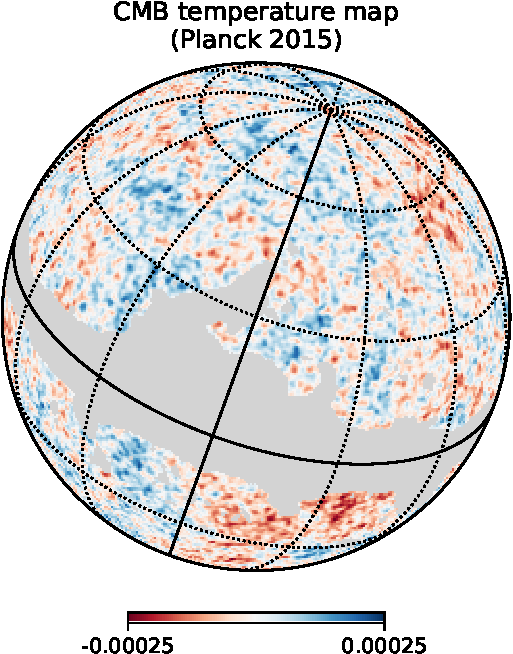
\includegraphics[height=0.3\linewidth]{example_cosmo_cmb}
	\hfill
	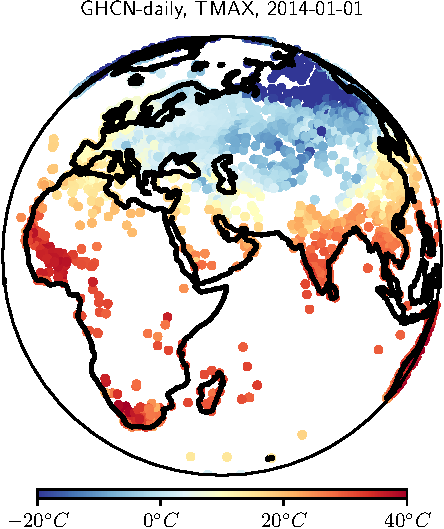
\includegraphics[height=0.3\linewidth]{example_ghcn_daily_tmax}
	\hfill
	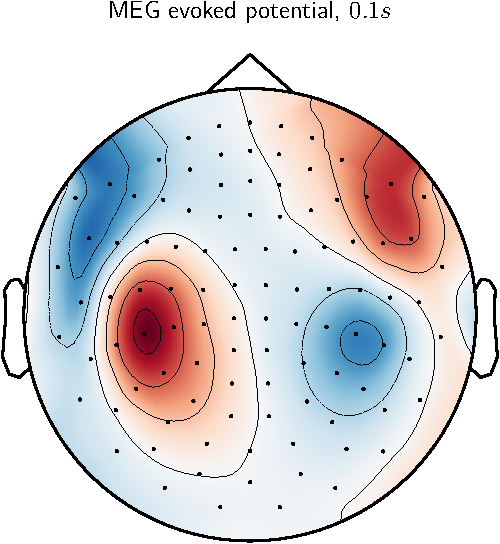
\includegraphics[height=0.3\linewidth]{example_brain_meg}
	\caption{
		Examples of real data on the sphere: (left) the cosmic microwave background (CMB) temperature from \citet{planck2015overview},
		%with galactic plane masked
		(middle) daily maximum temperature from the Global Historical Climatology Network (GHCN),\protect\footnotemark (right) brain activity recorded through magnetoencephalography (MEG).\protect\footnotemark
		For those examples, a rigid full-sphere pixelization is not ideal: the Milky Way's galactic plane masks observations, brain activity is measured on the scalp only, and the position and density of temperature sensors is arbitrary and changes over time.
		%\todo{something from climate, weather?}
		%\todo{compare ideal full-spheres (like SHREC-17 projection from Esteves, 360 from Coors) to real-world measurements?}
		%\todo{horizontal colorbar for brain}
	}
	\label{fig:examples}
\end{figure}
\footnotetext{\scriptsize\url{https://www.ncdc.noaa.gov/ghcn-daily-description}}
\footnotetext{\scriptsize\url{https://martinos.org/mne/stable/auto_tutorials/plot_visualize_evoked.html}}

\section{Introduction}

% \todo{sphere only, or start more general?}
% 1. general
% 2. sphere
% 3. equivariance to symmetries (we might not necessary want that)

% \todo{What is the problem we want to solve? Identify it. Our solution: flexible (any sampling) and computational efficient.}

% \todo{Related work: mention interest in spherical CNNs for various applications, importance of equivariance and invariance, previous exploratory work with graphs from Renata and ourselves.}

Graphs have long been used as models for discretized manifolds: for example to smooth meshes \citep{taubin1996meshsmoothing}, reduce dimensionality \citep{belkin2003laplacian}, and, more recently, to process signals \citep{shuman2013gsp}.
In most works, it is assumed that the true data manifold is unknown to the processing or learning method, and is only observed through discrete samples.
In this contribution, we want to make a case for using graphs as a support of computation on known manifolds.\footnote{For example, the plane where images live is known, while the true surface of a point cloud is unknown.}

%From now on, we focus on the sphere.
Along
%$d$-dimensional
Euclidean spaces, the sphere is one of the most commonly encountered manifold: it is notably used to represent omnidirectional images, global weather and climate data, cosmological observations, and brain activity measured on the scalp (see \figref{examples}).
Spherical convolutional neural networks (CNNs) have been developed to work with most of those modalities \citep{cohen2018sphericalcnn, esteves2017sphericalcnn, perraudin2018deepsphere, khasanova2017graphomni, boomsma2017sphericalcnn, su2017sphericalcnn, coors2018sphericalcnn,
% kondor2018sphericalcnn, => quite specific, same applications as Cohen
jiang2019sphericalcnn}.

% why graphs for the sphere
Spherical data can be seen as a continuous function
%$f: S^2 \rightarrow \R^d$
that is sampled at discrete locations.
%is sampled at convenient points, given by a chosen pixelization.
As it is impossible to construct a regular discretization of the sphere, there is no perfect spherical sampling.
Schemes have been engineered for particular applications and come with trade-offs \citep{gorski2005healpix,glesp}.
%emphasizing one or more features at the cost of others.
% For example, the equirectangular (a.k.a.\ equiangular or geographic) grid, used in most spherical CNNs, is most similar to a 2D grid.
% HEALPix features equal-area and hierarchically organized pixels, and has a fast spherical harmonic transform (SHT) \citep{healpix}.
% GLESP features a fast and exact
% %(to machine precision)
% SHT \citep{glesp}.
% sympix?, cubed-sphere? => no space
%\todo{maybe have a table, or a list of desired properties from a sampling} => no space
However, while sampling locations can be precisely controlled in some cases (like the CMOS sensors of an omni-directional camera), sensors might in general be non-uniformly distributed, cover only part of the sphere, and move (see \figref{examples}).
Modeling the sampled sphere as a discrete graph has the potential to faithfully and efficiently represent sampled spherical data by placing vertices where data has been measured: no need to handle missing data or to interpolate to some predefined sampling, and no waste of memory or precision due to over- or under-sampling.
Graph-based spherical CNNs have been proposed in \citet{khasanova2017graphomni} and \citet{perraudin2018deepsphere}.
Moreover, graph convolutions have a lower computational cost of $\bO(N_{pix})$ compared to $\bO(N_{pix}^{2/3})$ for the SHT-based convolutions of \citet{cohen2018sphericalcnn} and \citet{esteves2017sphericalcnn}, where $N_{pix}$ is the number of considered pixels.

%\todo{Most of our views are shaped by cosmology. What is going on in other fields (climate, weather)? Do they have their own samplings? Cosmo seems however the most advanced for SP on the sphere.}

%As the sphere $\mathcal{S}^2$ is a homogeneous space of the 3D rotation group $SO(3)$.

% Finally, to exploit the rotation symmetry of certain tasks involving spherical data, we would like a rotation equivariant formulation \citep{cohen2016equivariance}.
% speak about symmetries in the conclusion

Finally, like classical 2D CNNs are equivariant to translations, we want spherical CNNs to be equivariant to 3D rotations \citep{cohen2016equivariance, kondor2018equivariance}.
% we'll nuance this view in the conclusion
A rotation-equivariant CNN detects patterns regardless of how they are rotated on the sphere: they exploit the rotational symmetries of the data through weight sharing.
Realizing that, spheres can be used to support data which does not intrinsically live on a sphere but have rotational symmetries \citep[for 3D objects and molecules]{cohen2018sphericalcnn, esteves2017sphericalcnn}.
In this contribution we present DeepSphere~\cite{perraudin2018deepsphere}, a spherical neural network leaveraging graph convolution for its speed and flexibility. Furthermore, we discuss under which setting graph convolution on the sphere can is close to equivariant to rotations.

% \todo{From \citet{kondor2018equivariance}:
% A convolution implies the equivariance to the action of some group.
% Contrary as well: equivariance requires a convolution structure.
% }

% \begin{figure}
% 	% three figures: healpix, glesp, graph
% 	\label{fig:samplings}
% \end{figure}

\section{Method}

% \todo{Basics of GSP, how the graph is built, polynomial filters.}
Our method relies on the graph signal processing framework \cite{shuman2013gsp}. In this setting  


DeepSphere, presented in \figref{architecture}, leverages convolutions on graphs and hierarchical pooling to achieve the following properties: (i) computational efficiency(ii) adaptation to irregular sampling, and (iii) close to rotation equivariance,.
The main idea is to model the discretised sphere as a graph of connected pixels: the length of the shortest path between two pixels is an approximation of the geodesic distance between them.
We use the graph CNN formulation introduced in \citep{defferrard2016convolutional}, and a pooling strategy that exploits a hierarchical pixelisation of the sphere to analyse the data at multiple scales.
The current implementation of DeepSphere relies on the Equal Area isoLatitude Pixelisation (HEALPix)~\citep{gorski2005healpix}, a popular sampling used in cosmology and astrophysics.
DeepSphere is, however, easily used with other samplings as only two elements depend on it: (i) the choice of neighboring pixels when building the graph, and (ii) the choice of parent pixels when building the hierarchy.
The flexibility of modeling the data domain with a graph allows one to easily model data that spans only a part of the sphere, or data that is not uniformly sampled. 
Furthermore, using a $k$-nearest neighbours graph, the convolution operation costs $\mathcal{O}(N_{pix})$ operations, where $N_{pix}$ is the number of pixels.
This is the lowest possible complexity for a convolution without approximations.

Neverthless, while graphs offer great flexility, their ability to represent the underlying manifold (here the sphere) and hence for their convolution to be close to rotational equivariant will, as we shall see in the next section,  highly depends on sampling choice and on the graph construction.

% DeepSphere is readily apt to solve four tasks: (i) global classification (i.e., predict a class from a map), (ii) global regression (i.e., predict a set of parameters from a map), (iii) dense classification (i.e., predict a class for each pixel of a map), and (iv) dense regression, (i.e., predict a set of maps from a map).
% Input data are spherical maps with a single value per pixel, such as the CMB temperature, or multiple values per pixel, such as surveys at multiple radio frequencies.

% While there exists many graph NNs (see for example xxx and xxx for recent reviews),
% \todo{Why this graph NN? We want an equivalence with the continuous world to prove equivariance to arbitrary rotations.}

\begin{figure}
	\centering
	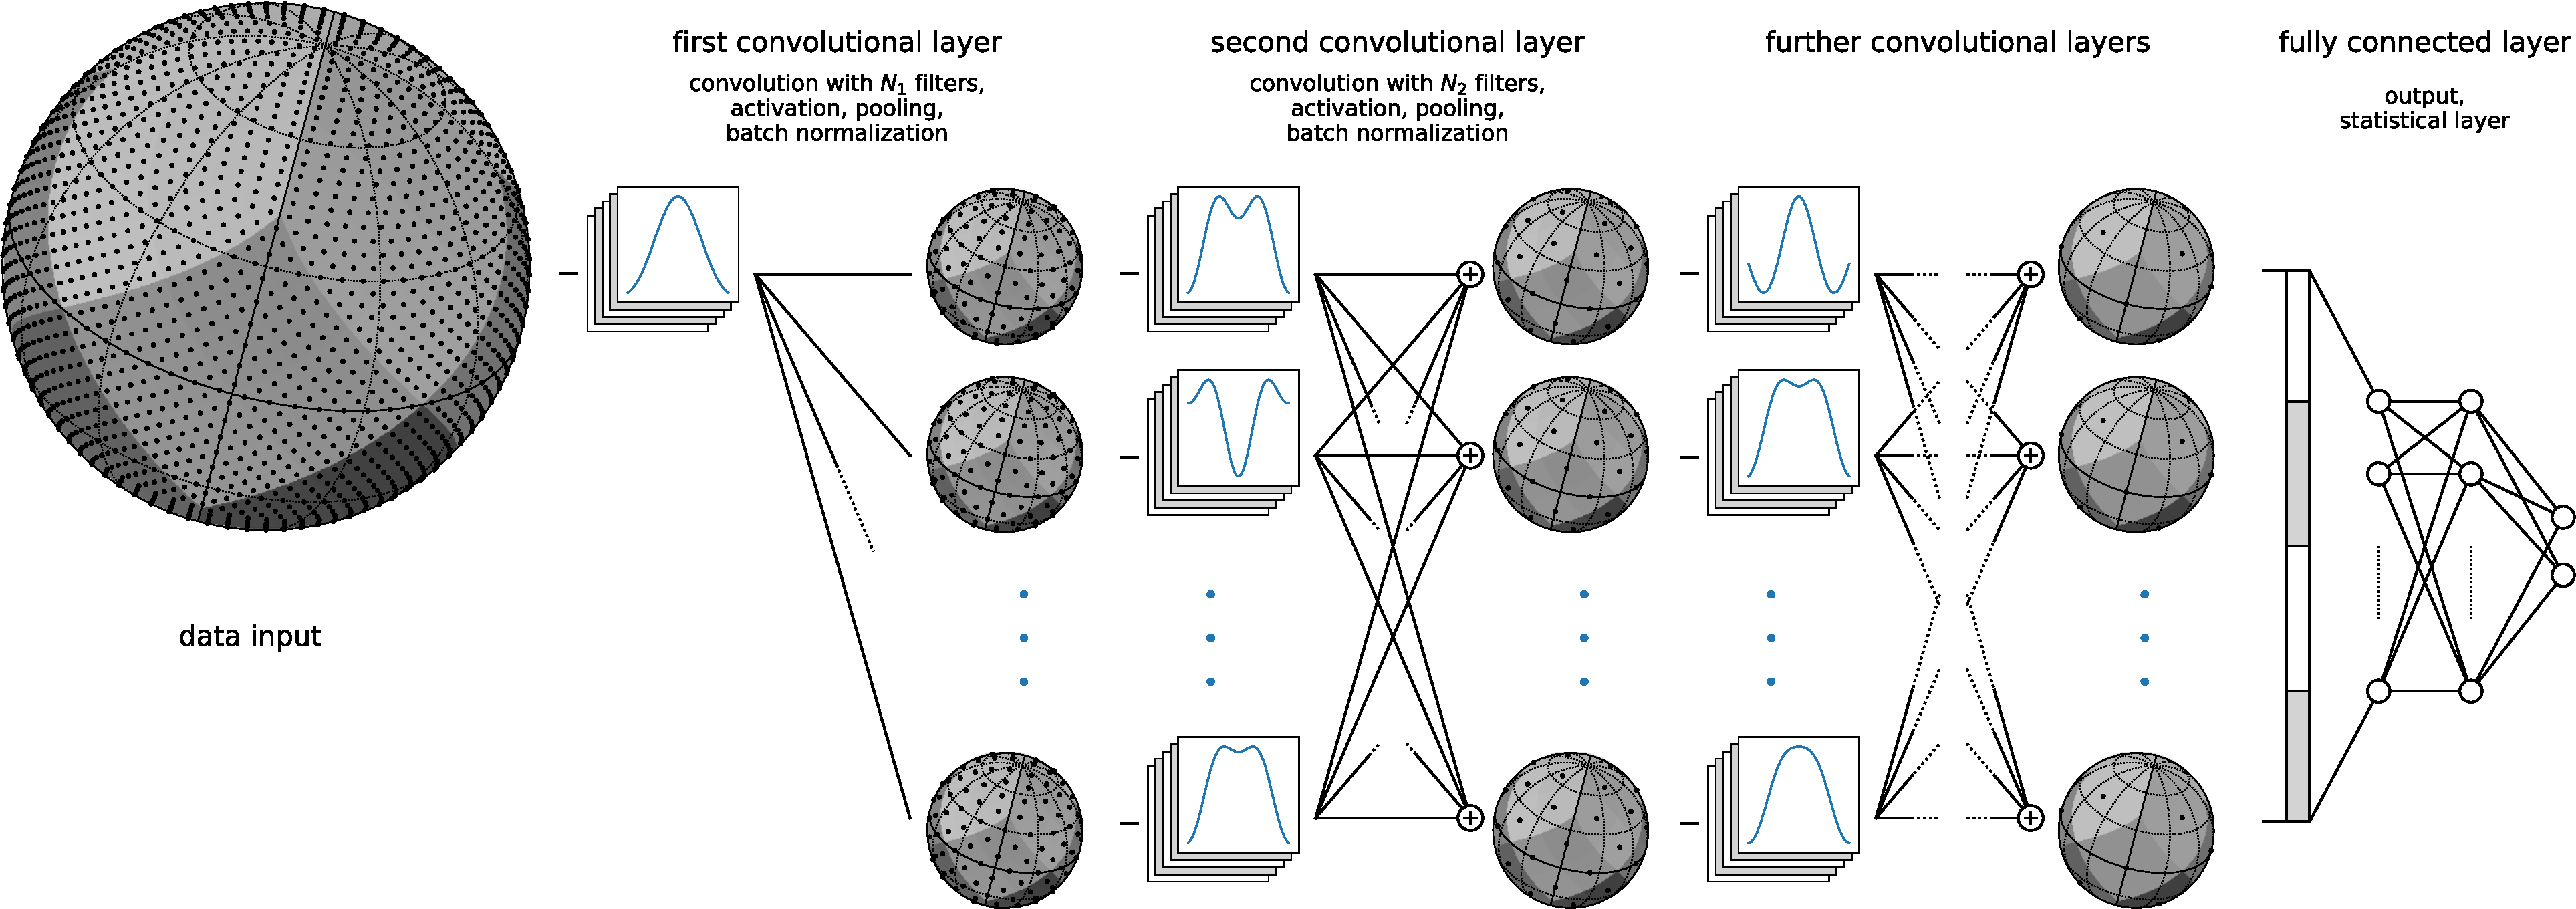
\includegraphics[width=\linewidth]{figure_architecture_v3}
	\caption{Overall NN architecture, showing here three convolutional layers acting as feature extractors followed by three fully connected layers with softmax acting as the classifier.
    A convolutional layer is based on five operations: convolution, non-linearity, batch normalization, down-sampling, and pooling.
	While most operations are agnostic to the data domain, the convolution and the down-sampling have to be adapted.
	In this paper, we propose first to model the sphere with a graph and to perform the convolution on the graph.
	Graphs are versatile data structures which can model any sampling, even irregular or partial.
	Second, we propose to exploit a hierarchical pixelization of the sphere for the down-sampling operation.
	It allows the NN to analyze the data at multiple scales while preserving the spatial localization of features.
	This figure shows a network that operates on the whole sphere.
	The process is the same when working with partial observations, except that the graph is only built for the region of interest.}
	\label{fig:architecture}
\end{figure}

% \todo{We can take here a different stance than: "we'll use whatever method gives the best performance". SHTs are the standard analysis tool on the sphere. People not only want to apply learned filters, but designed ones (e.g., Gaussian smoothing), people want to interpret and see the spectrum as spectral analysis is important (at least in cosmo, we should find some refs for that}





% That should be short: it's an ML audience. We can reference previous work. No general ML stuff, as in cosmo paper.

See \citet{perraudin2018deepsphere} for details.

%\section{Spherical harmonics and equivariance}
\section{Harmonics and equivariance}

% \todo{why equivalence to continuous provides equivariance. Clean way of doing it. Alternative: Renata's mechanical approach.}
% often easier to describe in Fourier space \citep{kondor2018equivariance} => motivation for the spectral interpretation?
% Proper study of symmetries and equivariance requires a continuous treatment.
% @Michael: Not necessarily. It is more complicated than that. For example, if you work in the spectral domain, you can bypass sampling problem. This is what happen with the work of Cohen. So I think we should not speak about that.
% For example, only rotations by $90^\circ$ can be studied on a discrete sampling grid.

% \todo{there is a compromise about the sampling quality (how far from uniform) and how close discrete computations can be made to the true continuous ones}

\begin{figure}
\centering
\begin{minipage}[c]{.21\textwidth}
	\centering
	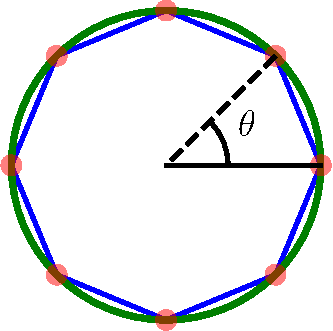
\includegraphics[width=\linewidth]{ring}
	\captionof{figure}{circle $\mathcal{C}^1$ (green), regularly sampled points and graph vertices (red), graph edges (blue).}
	\label{fig:ring}
\end{minipage}
\hfill
\begin{minipage}[c]{.7\textwidth}
	\centering
	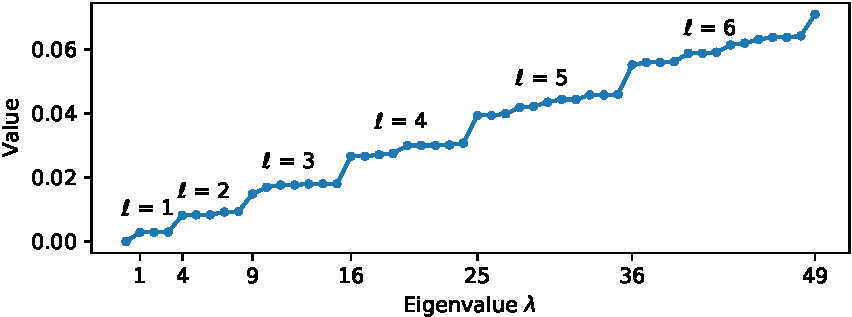
\includegraphics[width=\linewidth]{graph_eigenvalues}
	\captionof{figure}{The eigenvalues $\bLambda$ of the graph Laplacian $\L = \U \bLambda \U\trans$ are clearly organized in groups. Each group corresponds to a degree $\ell$ of the spherical harmonics. Each degree has $2\ell + 1$ orders.
	% See also \figref{graph_harmonics}.
	}
	\label{fig:graph_eigenvalues}
\end{minipage}
\end{figure}

\begin{figure}
	\centering
	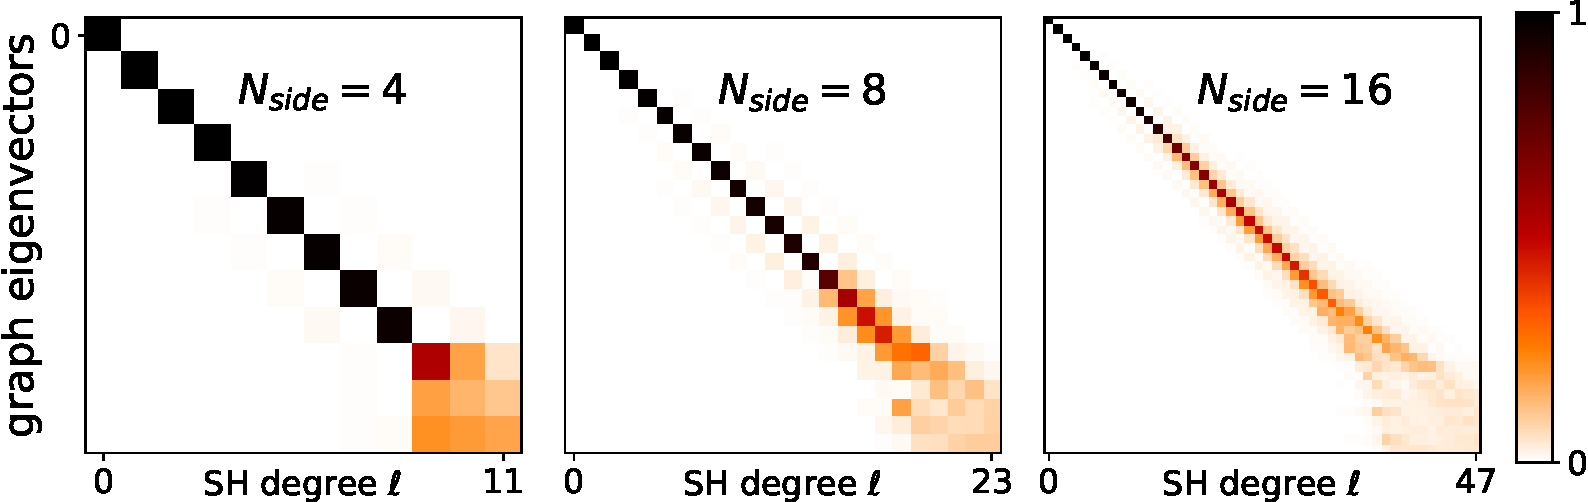
\includegraphics[width=0.9\linewidth]{subspace_harmonics_eigenvectors_v2}
	\caption{Correspondence between the subspaces spanned by the graph Fourier basis and the spherical harmonics.
		%The correspondence is computed in two steps.
		First, we compute the power spectral density (PSD) of each graph eigenvector.
		Second, as there is $2\ell+1$ spherical harmonics for each harmonic index $\ell$, we sum the contributions of the corresponding $2\ell+1$ graph eigenvectors.
		% No real convergence with increasing Nside.
		% Row $j$ is the sum of the (normalized) power spectral densities (PSDs), computed by the SHT, of the $2j+1$ graph Fourier modes $\b u_i$ identified with degree $j$.
		% The PSD is computed for degrees $\ell=0$ to $\ell = 3 N_{side} -1$.
		The matrix shows how the subspaces agree: the subspaces spanned by the Fourier modes correspond to those spanned by the spherical harmonics in the low frequencies, and the Fourier modes leak towards adjacent frequency bands at higher frequencies.
		%While there is a systematic error,
		The Fourier modes agree at higher frequencies as the resolution ($N_{side}$) increases.}
		\label{fig:subspace_harmonics_eigenvectors}
\end{figure}

%\paragraph{Why is the harmonic analysis of the graph important for equivariance?}
Both the graph and the spherical convolutions can be expressed as multiplications in a Fourier domain.
As the spectral bases align, the two operations become similar.
Hence, the equivariance property of the spherical convolution carries out to the graph convolution.
%the spectral analysis of the graph Laplacian gives insights on the equivariance property of the graph convolution.

\paragraph{Known case: the circle $\mathcal{C}^1$.}
Let $\theta\in[0,2\pi[$ be a parametrization of each point $(\cos\theta,\sin\theta)$ of $\mathcal{C}^1$.
The eigenfunctions of the Laplace-Beltrami operator of $\mathcal{C}^1$ are $u_\ell(\theta)=e^{i \theta m \ell}$, for $\ell \in \mathbb{N}$ and $m\in\{-1,1\}$.
Interestingly, for a \emph{regular sampling} of $\mathcal{C}^1$ (shown in \figref{ring}), the sampled eigenfunctions turn out to be the discrete Fourier basis.
That is, the harmonic decomposition of a discretized function on the circle can be done using the well-known discrete Fourier transform (DFT).
Moreover, the graph Laplacian of the sampled circle is diagonalized by the DFT basis, as all circulant matrices have complex exponentials as eigenbases \cite{strang1999dct}.
Hence, for $\mathcal{C}^1$, it can be verified, under mild assumptions, that the graph convolution is equivariant to translation \citep[section 2.2 and equation 3]{perraudin2017stationary}.
More generally, higher dimensional circles such as the torus $\mathcal{C}^2$ also have a circulant Laplacian and an equivariant convolution.
% For an irregular sampling however, the graph Fourier basis will not be the sampled eigenfunctions.
The above does however not hold for irregular samplings: the more irregular the sampling, the further apart the graph Fourier basis will be to the sampled eigenfunctions.
% Extreme case: all the samples at the same position.

% \paragraph{Necessary conditions for the rotational equivariance on the sphere}
% We note two important points for the equivariance property to be carried on the graph convolution: a) the sampling needs to be regular, and b), the constructed graph has to be constructed circulant,\footnote{A circulant graph is an undirected graph acted on by a cyclic group of symmetries which takes any vertex to any other vertex.} i.e. it has a circulant weight matrix.
% Unfortunately, there exist no regular sampling for a sphere $\mathcal{S}^2$ of more than $12$ points. Hence it is in general not possible to build a graph with a convolution that is equivariant to rotation\footnote{The exception is the dense graph. Unfortunately, in the extreme case the graph convolution is limited to Kronecker kernels, which makes it useless.}.



% \subsection{Boundary conditions}

% The graph setting used throughout this contribution corresponds to assumed reflective border conditions.
% While that is irrelevant when working on the complete sphere (as it has no border), it slightly affects the convolution operation when only a part of the sphere is considered.
% As depicted in \figref{border_effects}, a filter localized near a border (via $h(\L) \b \delta_i$) is no longer isotropic.
% These border effects can, however, be mitigated by padding with zeros a small area around the part of interest (in which case they become similar to border effects in classical CNNs).
% We however do not expect these effects to cause any problem as long as the data samples cover the same area.

% \begin{figure}[ht!]
% 	\centering
% 	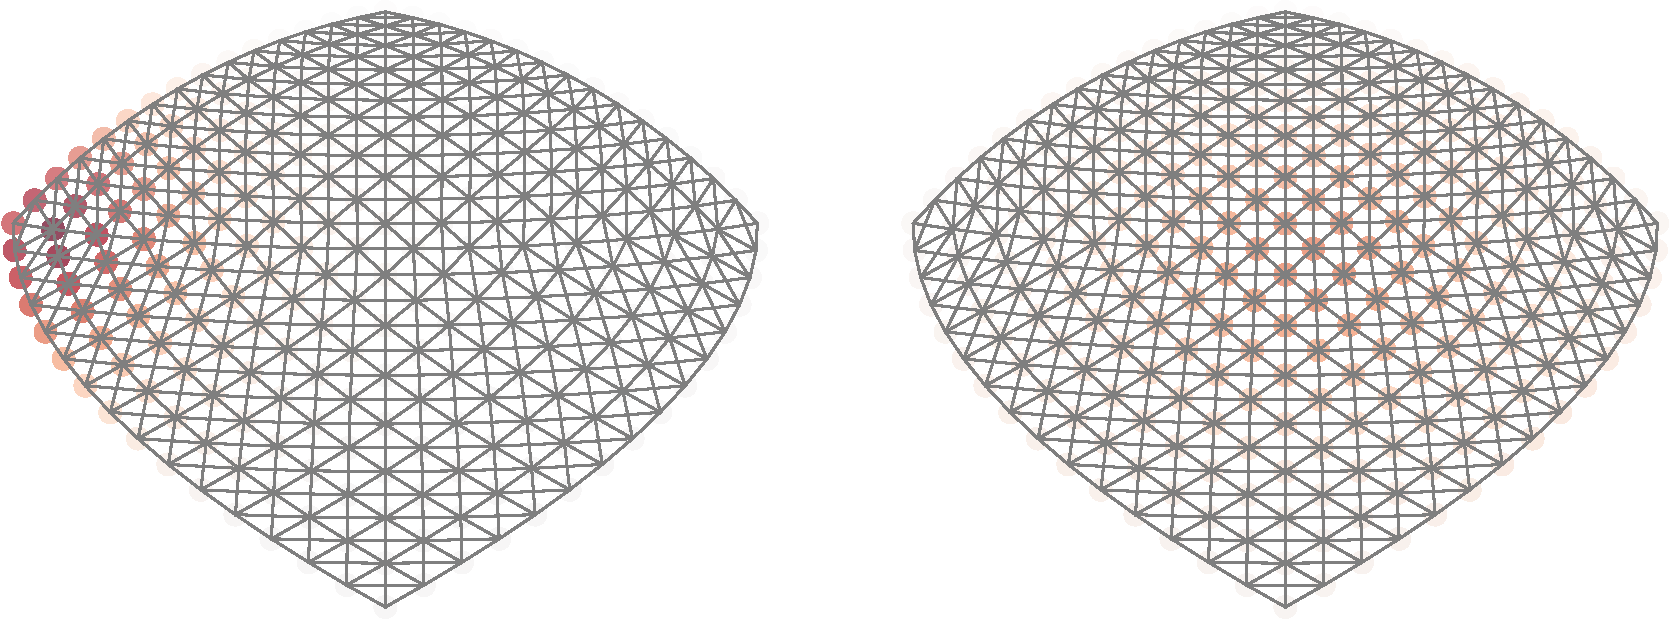
\includegraphics[width=\linewidth]{border_effects}
% 	\caption{Convolution kernel (also called filter) localized in the center and left corner of a graph built from $1/12^\text{th}$ of the sphere at $N_{side} = 16$.
% 		A filter $h$ is localized on a pixel $i$ as $\T_i h = h(\L) \b \delta_i$ (see \secref{graph_convolution}, equation~\eqnref{graph_convolution_spatial}).
% 	The filter is not isotropic anymore when localized on the corner as the graph representation of a manifold assumes reflective border conditions.}
% 	\label{fig:border_effects}
% \end{figure}


% \subsection{Convergence proof for random unform sampling}

% Let us use the angular parametrization of the sphere $\mathcal{S}^2=\{\bf{x} | \|\bf{x}\|_2=1 \}$, in term of angles of zenith, $\theta\in [0,\pi ]$, and azimuth $\phi\in [0,2\pi[$.
% \begin{equation}
% \Phi(\theta, \phi) = (\sin \theta \cos \phi, \sin \theta \sin \phi, \cos \theta )
% \end{equation}
% Let $\mathcal(C)^\infty(\mathcal{S}^2)$ denote the class of infinitely differentiable functions $\mathcal{S}^2\rightarrow \mathbb{R}$. Using the agnular parametrization of the sphere, the Laplace-Beltrami for a function $f\in \mathcal(C)^\infty(\mathcal{S}^2)$ is given by:
% \begin{equation}
% \Delta_{\mathcal{S}^2} f = \frac{1}{\sin \theta } \frac{\partial}{\partial \theta} \left(\sin \theta  \frac{\partial f}{\partial \theta} + \frac{1}{\sin^2 \theta} \frac{\partial^2f}{\partial \phi^2} \right)
% \end{equation}

% Let us extend the graph Laplacian

% \begin{equation}
% \L \b{f}[i] := \frac{1}{n} \left( \b{f}[i]\sum_{j=1}^n k_t(x_i,x_j) -\sum_{j=1}^n \b{f}[j] k_t(x_i,x_j)\right),
% \end{equation}
% where $k_t(x_i,x_j)=e^{-\frac{x_i-x_j}{4t}}$, \label{eq:full_graph_gaussian_weight}
% to each point on the Sphere.

%  It is a generalization of the graph Laplacian operator that apply on a function $f:\mathcal{S}^2 \rightarrow \mathbb{R} $:
% \begin{equation}
% L_t f(y) := \frac{1}{n} \left( f(y)\sum_{j=1}^n k_t(y,x_j)-\sum_{j=1}^n f(x_j)k_t(y,x_j) \right)
% \end{equation}


%  Given a function $f\in \mathcal{C}^\infty(\mathcal{S}^2)$ and for a fixed point $p \in \mathcal{C}^2$, after appropriate scaling the operator $L_t$, converge toward of the  Laplace–Beltrami operator.

% \begin{theorem}[Adaptation of Theorem 3.1 of~\cite{belkin2005towards}, Laplacian convergence] \label{theo:laplacian_convergence_belkin}
% Let data points $\b{x}_1,\dots, \b{x}_N$ be sampled from a uniform distribution on a manifold $\mathcal{M} \subset \mathbb{R}^T$.
% Using the weight function \eqref{eq:full_graph_gaussian_weight}, define a sequence $t_N=N^{-\frac{1}{4+\alpha}}$, where $\alpha>0$ and let $f\in \mathcal{C}^\infty(\mathcal{C}^2)$, then the following holds:
% \begin{equation}
% \lim_{N \rightarrow \infty} \frac{1}{t_N(4\pi t_N)} (L \b{f})[i] = \frac{1}{\text{vol} (\mathcal{C}^2)} (\Delta_{\mathcal{C}^2} f)(\b{x}_i)
% \end{equation}
% where the limit is taken in probability and $\text{vol}(\mathcal{C}^2)=4 \pi$ is the surface of the sphere with respect to the canonical measure.
% \end{theorem}

% \subsection{Empirical analysis of the graph eigenvectors}

% The first 16 eigenvectors $[\b u_1, \ldots, \b u_{16}]$ of the graph Laplacian $\L$, forming the lower part of the graph Fourier basis $\U$, are shown in \figref{graph_harmonics}.

\paragraph{Empirical analysis of the graph Laplacian used in DeepSphere.}
% Let us further observe the spectral properties of our constructed spherical graph laplacian $\L$.
%Given the graph used for DeepSphere, let us analyze the spectral alignment of the graph Fourier basis and the spherical harmonics.
The graph Laplacian eigenvalues, shown in \figref{graph_eigenvalues}, are clearly organized in frequency groups of $2\ell + 1$ orders for each degree $\ell$.
These blocks correspond to the different eigenspaces of the spherical harmonics.
We also show the correspondence between the subspaces spanned by the graph Fourier basis and the spherical harmonics in \figref{subspace_harmonics_eigenvectors}.
For $N_{side}=4$, we clearly observe a good alignment for $\ell \leq 8$: the graph convolution will be equivariant to rotations for low frequency filters.
The imperfection in the alignment is likely due to the small irregularities in the HEALPix sampling (varying number of neighbors and varying distances).
Furthermore, the graph construction is most probably not optimal.
% as the resulting Laplacian is probably far from circulant.
%One construction scheme that might be more adapted is a fully connected graph as this scheme is used in convergence proof in \cite{belkin2005towards,belkin2007convergence}.
% Those discrepancies result in a convolution operation that is not exactly equivariant to rotation.
% Nevertheless, our experiments suggest that these downsides do not have an important effect on the convolution nor hinder the performance of the NN.

% \todo{new results from Martino: becomes better in BN setting, currently under study}

\todo{we have less rich operations (compared to the most general linear equivariant map) by restricting our filters to be radial, but does it matter in practice?}
\todo{isotropic filters provide invariance to the third rotation}

\section{Experiments}

\todo{the cosmo experiment}

Preliminary results on shape retrieval (SHREC-17) indicate similar performance as \citet{cohen2018sphericalcnn} and \citet{esteves2017sphericalcnn}.
\todo{(while being isotropic and invariant to the third rotation)}

% \begin{figure}
% 	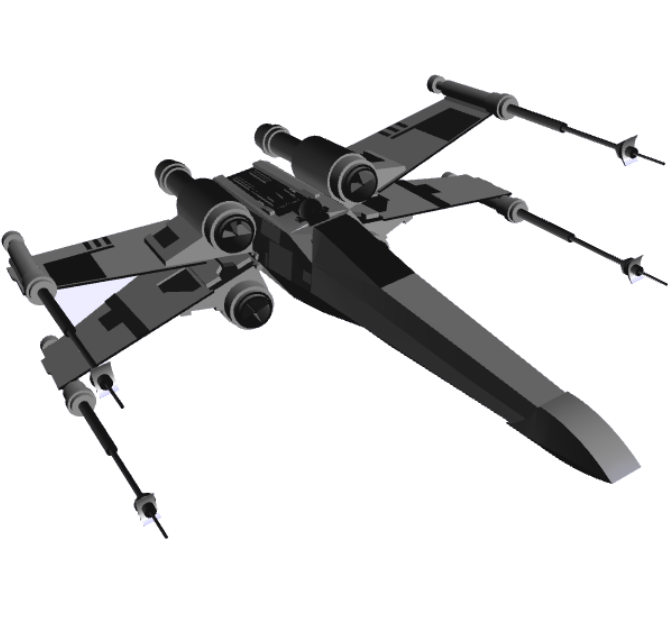
\includegraphics[height=0.2\linewidth]{example_model_esteves}
% 	\includegraphics[height=0.2\linewidth]{example_model_projected_esteves}
% 	\caption{
% 		Projection of a 3D model on the sphere.
% 		Typical task on which spherical CNNs are evaluated.
% 		Compared to the examples in \figref{spherical_data_examples}, the data covers the whole sphere and is regularly sampled.}
% \end{figure}

\section{Conclusion}  % & perspective

\todo{Generalization vs specialization: most general is to assume no symmetries (fully connected NN).
NNs can be specialized by adding some equivariance and invariance to symmetry groups such as translation, rotation, flip, etc.
More specialized NNs are more limited in the class of functions they can approximate, but requires less samples.
Again, use the right symmetries.}

exploit symmetries in the data by being equivariant (or invariant) to a select group of symmetric transformations (symmetry group).
In this paper, we argue that graph neural networks are a flexible model (albeit not the most general) to exploit such symmetries.

\todo{As equivariance is not the Graal either. We expect the desired amount of equivariance to depend on the data and task. As usual, practitioners should adopt a NN architecture that exploit the symmetries of their problem. \citep{coors2018sphericalcnn, jiang2019sphericalcnn}.}

\todo{future directions: equivalence / convergence to spherical harmonics, other tasks, comparison with other spherical CNNs, graph CNNs (especially those for manifolds), boundary conditions on partial sphere}

\textbf{Long term vision.}

We hope to establish graphs as a generic support for processing and learning over known and unknown manifolds.
\todo{Applications are plenty:
known manifolds (1D, 2D, 3D Euclidean spaces, circle, sphere)
% Minkowski spacetime
unknown manifolds (shapes, point clouds, feature sets)
}
\todo{
* known manifolds: grid, sphere, spacetime (a pseudo-Riemannian 4-manifold), surfaces defined by NURBS, anything else?
* unknown manifolds: meshes (human body), point clouds => what are the symmetries? local isometry
* non-manifold: all networks (brain, social, transportation, telecom, etc.) and relations (author-papers, user-products)
}

\todo{Similar goal: graph CNNs for group equivariant convolution.}

The vision is to push the use of graphs as the support for computation on manifolds. The advantages of graphs are to relax constraints on the sampling (e.g., allow an irregular or partial sampling), and be computationally more efficient (while being exact w.r.t. the continuous case).
Part of a broader research effort to explore the use of GSP to solve continuous problems.

\subsubsection*{Acknowledgments}

\todo{Pierre, Cardoso, Tomek?}

\bibliography{refs}
\bibliographystyle{iclr2019}

\end{document}
